%%% Exemplo de utiliza��o da classe ITA
%%%
%%%   por        F�bio Fagundes Silveira   -  ffs [at] ita [dot] br
%%%              Benedito C. O. Maciel     -  bcmaciel [at] ita [dot] br
%%%              Giovani Volnei Meinertz   -  giovani [at] ita [dot] br
%%%
%%%  IMPORTANTE: O texto contido neste exemplo nao significa absolutamente nada.  :-)
%%%              O intuito aqui eh demonstrar os comandos criados na classe e suas
%%%              respectivas utilizacoes.
%%%
%%%  $Id: ExemploTeseITA.tex 17 2006-02-07 17:59:17Z ffs $
%%%  $HeadURL: file:///opt/repositorioITALUS/classeITA/tags/versao-2.1/ExemploTeseITA.tex $
%%%
%%% ITALUS
%%% Technological Institute of Aeronautics --- ITA
%%% Sao Jose dos Campos, Brazil
%%% HomePages:        http://www.comp.ita.br/italus
%%%                   http://groups.yahoo.com/group/italus/
%%% Discussion list: italus {at} yahoogroups.com
%%%
%++++++++++++++++++++++++++++++++++++++++++++++++++++++++++++++++++++++++++++++
% Parametros da classe ITA:
%   msc   = Tese de Mestrado    --> no ITA, Dissertacao eh Tese ...  :-)
%   dsc   = Tese de Doutorado
%   quali = Exame de Qualificacao
%   dv    = 'Draft Version'     --> imprime 'Versao Preliminar + data no rodape
%   fem   = Doutora
%   eng   = para teses em ingl�s
%++++++++++++++++++++++++++++++++++++++++++++++++++++++++++++++++++++++++++++++
\documentclass[msc]{ita}    % ITA.cls based on standard book.cls

%++++++++++++++++++++++++++++++++++++++++++++++++++++++++++++++++++++++++++++++
% Identificacoes...
%++++++++++++++++++++++++++++++++++++++++++++++++++++++++++++++++++++++++++++++
\course{Engenharia Eletr�nica e Computa��o}
\dept{Ci�ncia da Computa��o}
\area{Inform�tica}

% Autor do trabalho: Nome Sobrenome
\author{Bruno}{Duarte Corr�a}

% Endereco do Autor -> utilizado no verso da folha de rosto
% Obrigat�rio para Teses
\itaauthoraddress{Av. ABC, 1000}{12.000-000}{S�o Jos� dos Campos--SP}

% Titulo da Tese/Dissertacao
\title{Como produzir teses e disserta��es com o estilo ITALUS}

% Orientador
\advisor{Prof.~Dr.}{Fulano de Tal}

% Co-orientador opcional
\coadvisor{Prof.~Dr.}{Beltrano de Tal}{OVNI}

% Chefe da divisao de Pos-Graduacao
% Obrigat�rio para Teses
\boss{Prof.~Dr.}{Cicrano de Tal}

% Banca Examinadora
% Obrigat�rio para Teses
\examiner{Prof. Dr.}{Fulano Beltrano}{Presidente}{ITA}%
\examiner{Prof. Dr.}{Cicrano Fulano}{Membro Externo}{UXXX}%
\examiner{Prof. Dr.}{Beltrano Cicrano}{Membro Externo}{UYYY}%
\examiner{Prof. Dr.}{Fulano de Tal}{Membro}{ITA}%
\examiner{Prof. Dr.}{Beltrano Fulano}{Membro}{ITA}%

% Data da defesa
\date{Fevereiro}{2015}

% Palavras-Chaves informadas pela Biblioteca -> utilizada na CIP
% Obrigat�rio para Teses
\kwcip{Teses}
\kwcip{Estilos}
\kwcip{Italus}

% Glossario
\makeglossary
\frontmatter

\begin{document}

% Folha de Rosto
\maketitle

% Dedicatoria
\begin{itadedication}
Aqui pode ser escrita uma dedicat�ria. N�o � obrigat�ria.
\end{itadedication}

% Agradecimentos
\begin{itathanks}
\input{parts/agradecimentos}
\end{itathanks}

% Ep�grafe
\thispagestyle{empty}
\ifhyperref\pdfbookmark[0]{\nameepigraphe}{epigrafe}\fi
\begin{flushright}
\begin{spacing}{1}
\mbox{}\vfill
{\sffamily\itshape
``If I have seen farther than others,\\
it is because I stood on the shoulders of giants.''\\}
--- \textsc{Sir~Isaac Newton}
\end{spacing}
\end{flushright}

% Resumo
\begin{abstract}
O reconhecimento de objetos em uma cena para posterior uso em realidade aumentada 
depende de diversas vari�veis, causando a necessidade do uso de t�cnicas 
espec�ficas para cada cen�rio, sendo portanto, um estudo de fronteiras para a melhor escolha 
do algoritmo de reconhecimento, de acordo com a aplica��o em quest�o de grande
valia para o meio acad�mico. 
Esta tese se prop�e a pesquisar, categorizar e tra�ar fronteiras das t�cnicas
conhecidas, tendo como caso de uso a manuten��o de aeronaves feita dentro de
centros fechados, utilizando as t�cnicas BRISK,FAST,FREAK,GFTT,MSER,
 ORB,STAR,SURF,SIFT em uma an�lise aplicada com imagens reais de janelas de
 inspe��o do Embraer ERJ-190 para reconhecimento de objetos e posteriores
 aplica��es em manuten��o.
 Comparando todas as t�cnicas quanto � cad�ncia e � precis�o de reconhecimento
 de caracter�sticas, � poss�vel selecionar GFTT e ORB
 como t�cnicas mais apropriadas ao contexto, por terem seus resultados de
 varia��o de rota��o, escala, briho e \emph{blur} dentro de uma faixa esperada
 para o contexto de manuten��o.
 


\end{abstract}
% Palavras Chave
% No manual nao consta palavras-chaves
%\keywords{Teses, Estilos, Italus}

% Abstract
\begin{englishabstract}
Recognition of objects in a scene for later use in augmented reality depends on several variables, causing the need 
to use several specific techniques for each scenario, and therefore a border
analysis to the best choice of the registration algorithm according to
application in question, of great value to academia.
This thesis aims to examine, categorize and draw boundaries of the known techniques having as use case maintenance of 
aircraft made in closed center, using the techniques BRISK,FAST,FREAK,GFTT,MSER,
ORB,STAR,SURF,SIFT in an applied analysis with images of the Embraer ERJ-190 to recognition of objects and future usage in maintenance. Comparing all of the techniques, using cadency and recognition precision, it is possible to chose GFTT and ORB as the most appropriate ones because its results to the variation of
rotation, scale, brightness and blur fulfils the constraints needed

\end{englishabstract}
% Keywords
% Idem Palavras-chaves ...
%\englishkeywords{Theses, Styles, Italus}

% sumario
\tableofcontents
% lista de figuras
\listoffigures
% lista de tabelas
\listoftables
% lista de abreviaturas
\listofabbreviations
 \begin{table}[H]
  \centering
      \caption{Lista de Acr�nimos}
\label{table:acronym}
    \begin{tabular}{ll}
    AR   & Augmented Reality      \\
    BRIEF & Binary Robust Independent Elementary Features\\
    BRISK & Binary Robust Invariant Scalable Keypoints\\
    DoG  & Difference of Gaussians \\
	FAST & Features from Accelerated Segment Test\\
    FREAK & Fast Retina Keypoint\\
    GFTT & Good Features To Track\\
    GPU & Graphics Processing Unit \\
     HMD & Head-Mounted Display   \\
    LoG  & Laplacian of Gaussians  \\
    MSER & Maximally Stable Extremal Regions\\      
   ORB & Oriented Fast and Rotated Brief\\

    SIFT & Scale-Invariant Feature Transform\\
    SURF & Speed Up Robust Feature\\
    STAR & N�o � um acr�nimo\\ 
    VR   & Virtual Reality        \\
    
   
    
    
    
    
    \end{tabular}

\end{table}


% lista de simbolos
%\listofsymbols
%\input{parts/listasimbolos}

\mainmatter
% Os capitulos comecam aqui

\chapter{Motiva��o}
O reconhecimento de estruturas e sistemas de forma autom�tica no campo da manuten��o  auxilia al�m de garantir maior confiabilidade no diagn�stico de problemas pode propiciar uma ferramenta de capacita��o entre v�rias possibilidades.
Um dos mais b�sicos problemas atualmente limitando o ramo da Realidade Aumentada � a etapa de registro.
A Realidade Aumentada prev� imers�o entre o mundo virtual e o mundo real e por isso para que a experi�ncia de imers�o seja coerente � necess�rio que os dois mundos estejam bem sincronizados e propriamente alinhados. Para algumas aplica��es tal sincronia aumenta a experi�ncia, entretanto existem aplica��es que tal alinhamento � primordial, por exemplo em aplica��es m�dicas por exemplo em uma aplica��o de biopsia.Se o objeto n�o estiver no espa�o e tempo da realidade, a informa��o fornecida ao cirurgi�o poder� por em risco a vida do paciente. Na maioria das aplica��es de tempo real, problemas de registro podem invalidar o uso da Realidade Aumentada.
Um outro problema que pode ocorrer com falhas de registro � acentuado por um fen�meno conhecido como visual capture[Welch78] que � a tend�ncia do c�rebro acreditar mais no que v� do que no que sente, ouve, etc. Nesses casos o sentido da vis�o tende a sobrepor os outros sentidos.
Assim como um ventr�loco consegue enganar que assiste um show acreditando que o som sai da boca do boneco o usu�rio de uma aplica��o de realidade aumentada tender� a acreditar no que v�, mesmo que esteja defasado no espa�o/tempo.
No caso do erro se tornar sistem�tico o usu�rio tende a se acostumar inconscientemente e se adaptar ao erro, corrigindo o efeito
Erros de registro s�o dif�ceis de controlar adequadamente devido � grande precis�o requerida das diversas fontes de erro. As fontes de erro podem ser divididas em est�ticas e din�micas sendo as est�ticas contornadas com calibra��o pr�via de sensores entretanto os erros din�micos s�o mais dif�ceis porque s�o suscept�veis a tempo diferen�a de tempo entre o real e o apresentado na tela e com o ac�mulo de erro.
O reconhecimento de objetos na cena permeia tamb�m:
\begin{itemize}
  \item O contexto da cena, sendo que com conhecimento pr�vio do cen�rio se torna bem mais f�cil;
  \item O material do qual o objeto � feito, porque caso seja feito de materiais reflexivos, os algoritmos podem confundir o reflexo de outros objetos com informa��es a reconhecer;
  \item 	O tamanho do objeto, pois de acordo com a escala do objeto, muitas informa��es que poderiam ser boas para o reconhecimento podem estar pr�ximas demais dificultando o posteior casamento de informa��es. \ldots
\end{itemize}

Portanto para que as diversas fontes de erros din�micos n�o sejam um impeditivo para o reconhecimento, de acordo com a cena, algoritmos diferentes devem ser selecionados por terem peculiaridades e caracter�sticas que garantam um registro direcionados ao tipo de desafio que encontrar�o, al�m de j� ter informa��es pr�vias, o que facilita na sele��o de caracter�sticas.



\chapter{Objetivo}
O presente trabalho tem como objetivo geral avaliar o ambiente de manuten��o aeron�utico interno, no contexto de janelas de inspe��o e tra�ar estrat�gias de reconhecimento de items de manuten��o.
Para a consecu��o do objetivo geral, foram definidos os seguintes objetivos espec�ficos:


\begin{itemize}
\item Avaliar as algoritmos cl�ssicos de reconhecimento;
\item Levantar caracter�sticas padr�o dos objetos no contexto;
\item Avaliar limites de percep��o humanas das caracter�sticas padr�o;
\item Avaliar algoritmo mais adequado para o contexto.
\end{itemize}
	
A proposta dessa tese � a partir do cen�rio de manuten��o de aeronaves e da proposta de utiliza��o de realidade aumentada, determinar a melhor estrat�gia de reconhecimento de pe�as para que posteriormente seja utilizado em ferramentas de auxilio na manuten��o por meio da realidade aumentada

\cite{ISMAR2012}
\cite{ORB}


\chapter{Restri��es}
\section{Vari�veis de contorno}
\label{sec:variaveiscontorno}
O cen�rio de reconhecimento de objetos dentro da aeronave traz alguns desafios que devem ser contornados
\begin{itemize}
\item Pouca ilumina��o em ambientes internos
\item Objetos muito parecidos entre si
\item Alguns objetos com textura
\item Objeto brilhante
\end{itemize}
\section{Restri��es}
\label{sec:restricao}

O contexto dessa tese prev� o cen�rio de manuten��o com o uso de realidade aumentada como uma ferramenta para auxiliar nas tarefas rotineiras portanto algumas vari�veis devem ser consideradas para garantir a viabilidade de implanta��o da abordagem:
\begin{itemize}
\item Velocidade de reconhecimento
\item Qualidade do reconhecimento
\item Invari�ncia quanto � par�metros ambientais
\end{itemize}

\chapter{Conceitos}
\subsection{Realidade Aumentada}
A realidade aumentada � uma t�cnica de vis�o computacional em que valendo-se de artefatos do mundo real tem por objetivo causar sensa��o de imers�o do usu�rio em um ambiente aumentado por artefatos virtuais, ao contr�rio de ambientes puramente virtuais como � comum em aplica��es de realidade virtual.
Idealmente o mundo virtual se torna imersivo o suficiente para que o usu�rio n�o consiga distinguir o real do virtual.
Alguns autores definem AR como tendo a necessidade de utilizar-se interfaces visuais port�teis para que a usabilidade tenha mais coer�ncia com a proposta inicial de garantir uma experi�ncia imersiva.
As imagens s�o obtidas por c�meras e o resultado apresentado em dispositivos como projetores ou displays como monitores, tablets ou head-mounted display (HMD).
\subsection{Head-Mounted Displays}
� um equipamento utilizado na cabe�a de forma que as duas m�os do usu�rio fiquem livres e tem por objetivo exibir imagens e �udio, sendo uma interface muito utilizada tanto em RV quanto em RA.
Os HMD basicamente s�o dispositivos constitu�dos de duas telas posicionadas frente ao olho do usu�rio.
Com duas telas, a tecnologia pode ser empregada para exibir imagens estereosc�picas apresentando os respectivos pontos de vista de cada olho para cada tela, o que contribui em muito na experi�ncia de imers�o.
Os HMDs funcionam tamb�m como dispositivos de entrada de dados, porque cont�m sensores de rastreamento que medem a posi��o e orienta��o da cabe�a, transmitindo esses dados ao computador.
Existem dois tipos de HMDs: Feed-Through e See-Through
\subsubsection{Feed-Through}
S�o dispositivos que � um sistema fechado de visualiza��o de imagens, em que o usu�rio consegue enxergar somente o que � mostrado no display, sendo assim o resultado apresentado � sempre a soma da imagem real com informa��es superpostas

\begin{figure}[h!]
\centering
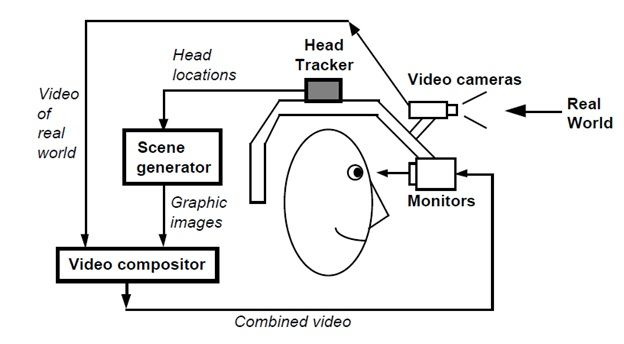
\includegraphics[scale=0.7]{images/feedthrough}
\caption{Arquitetura do Feed-Trough.}
\label{feedthrough}
\end{figure}


\subsubsection{See-Through}
S�o dispositivos constru�dos com lentes transl�cidas em que o usu�rio enxerga o mundo real e com algum tipo de sistema que sobrepoe na lente as informa��es adicionais

\begin{figure}[h!]
\centering
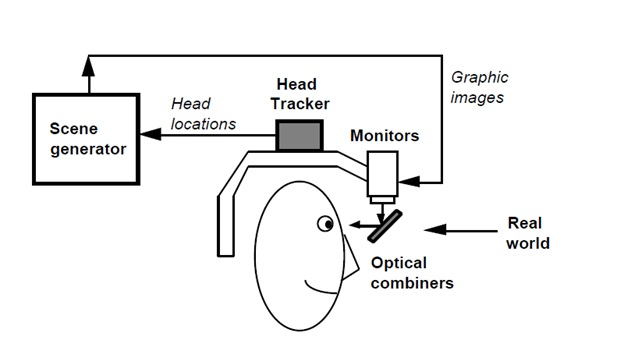
\includegraphics[scale=0.7]{images/seethrough}
\caption{Arquitetura do See-Trough.}
\label{seethrough}
\end{figure}


\subsubsection{Projetores}
O uso de projetores possibilita uma abordagem de realidade aumentada diferente porque pode ser utilizada para cobrir superf�cies largas, projetando sobre objetos como carros, pessoas, pr�dios, etc�.
Um problema dessa abordagem � que a calibra��o se faz necess�ria em v�rias situa��es.

\subsubsection{Monitores}
O uso de monitores reduz bastante o custo da aplica��o apesar de ter perda de imers�o por ser um m�todo de visualiza��o indireta, o que implica o usu�rio ficar olhando na dire��o do monitor, entretanto existe a possibilidade de compartilhar os resultados da RA com mais de uma pessoa ao mesmo tempo.

\begin{figure}[h!]
\centering
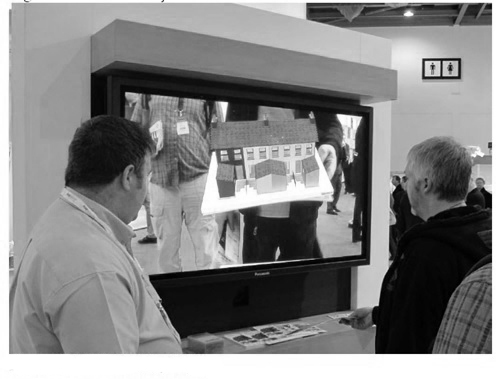
\includegraphics[scale=0.7]{images/monitores}
\caption{Realidade Aumentada com projetores.}
\label{monitores}
\end{figure}

% Referencias Bibliograficas
\begin{spacing}{1.0}
\begin{flushleft}
\bibliography{refs_exemplo}
\end{flushleft}
\end{spacing}


% Apendices
%\appendix
%\chapter{T�picos de �lgebra Linear}
%\input{apendiceA}

% Anexos
%\annex
%\chapter{Exemplo de um Primeiro Anexo}
%\input{anexoA}

% Glossario
\itaglossary
\printglossary

% Folha de Registro do Documento
% Valores dos campos do formulario
\FRDitadata{24 de dezembro de 1969}
\FRDitadocnro{CTA/ITA - IEC/TM-002/1969}
\FRDitaorgaointerno{Divis�o de Ci�ncia da Computa��o -- ITA/IEC}
\FRDitapalavrasautor{Teses; Estilos; Italus}
\FRDitapalavrasresult{Teses e Disserta��es; Estilos; Usu�rios}
\FRDitaresumo{O reconhecimento de objetos em uma cena para posterior uso em realidade aumentada 
depende de diversas vari�veis, causando a necessidade do uso de t�cnicas 
espec�ficas para cada cen�rio, sendo portanto, um estudo de fronteiras para a melhor escolha 
do algoritmo de reconhecimento, de acordo com a aplica��o em quest�o de grande
valia para o meio acad�mico. 
Esta tese se prop�e a pesquisar, categorizar e tra�ar fronteiras das t�cnicas
conhecidas, tendo como caso de uso a manuten��o de aeronaves feita dentro de
centros fechados, utilizando as t�cnicas BRISK,FAST,FREAK,GFTT,MSER,
 ORB,STAR,SURF,SIFT em uma an�lise aplicada com imagens reais de janelas de
 inspe��o do Embraer ERJ-190 para reconhecimento de objetos e posteriores
 aplica��es em manuten��o.
 Comparando todas as t�cnicas quanto � cad�ncia e � precis�o de reconhecimento
 de caracter�sticas, � poss�vel selecionar GFTT e ORB
 como t�cnicas mais apropriadas ao contexto, por terem seus resultados de
 varia��o de rota��o, escala, briho e \emph{blur} dentro de uma faixa esperada
 para o contexto de manuten��o.
 

}
%  Primeiro Parametro: Nacional ou Internacional -- N/I
%  Segundo parametro: Ostensivo, Reservado, Confidencial ou Secreto -- O/R/C/S
\FRDitaOpcoes{N}{S}
% Cria o formulario
\itaFRD

\end{document}
% Fim do Documento.
